\documentclass{article}
\usepackage[utf8]{inputenc}
\usepackage{graphicx}
\usepackage{amsmath}
\usepackage{amsfonts}
\usepackage{amssymb}
\usepackage{xcolor}
\usepackage{geometry}
\usepackage{caption}
\usepackage{listings} % Per blocchi di codice

\geometry{a4paper, margin=1in}

\title{Documentazione del Metodo TIMO}
\date{\today}

\lstset{
  basicstyle=\ttfamily\footnotesize,
  breaklines=true,
  frame=single,
  language=Python, % Linguaggio di default per i blocchi di codice
  keywordstyle=\color{blue},
  commentstyle=\color{green!40!black},
  stringstyle=\color{purple},
  showstringspaces=false
}

\begin{document}
\maketitle
\tableofcontents
\newpage

\section{Introduzione a TIMO}
TIMO è un approccio sviluppato nell'ambito del \textit{few-shot learning} che sfrutta modelli pre-addestrati come CLIP (Contrastive Language-Image Pre-training). L'obiettivo è migliorare la classificazione di immagini utilizzando un numero molto limitato di esempi di training per classe. TIMO opera principalmente estraendo e raffinando feature visive e testuali, per poi utilizzarle in un processo di classificazione. Il codice fornito, in particolare \texttt{main.py} e \texttt{extract\_features\_all.py}, illustra il flusso di lavoro di TIMO e lo confronta con altri metodi \textit{state-of-the-art} come Tip-Adapter, APE e GDA-CLIP.

La Figura \ref{fig:timo_overview} mostra uno schema generale del funzionamento di TIMO.

\begin{figure}[h!]
    \centering
    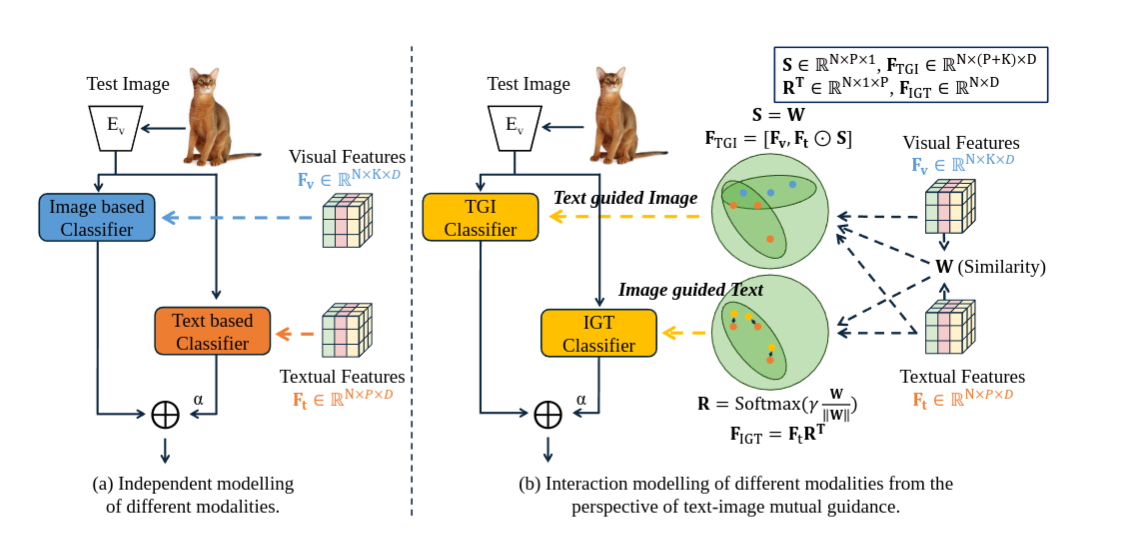
\includegraphics[width=0.8\textwidth]{TIMO.png}
    \caption{Schema generale del framework TIMO.}
    \label{fig:timo_overview}
\end{figure}

\section{Ruolo e Utilizzo dei Set di Dati}
TIMO, come molti approcci di machine learning, utilizza distinti set di dati per l'addestramento, la validazione e il test. La gestione di questi set è cruciale per il corretto funzionamento e la valutazione del metodo.

\subsection{Training Set (Few-Shot)}
Il training set in TIMO è tipicamente un set \textit{few-shot}, il che significa che contiene solo un numero limitato di esempi per ogni classe (ad esempio, 1, 2, 4, 8, o 16 campioni, come specificato dall'argomento \texttt{--shot} e dalla variabile \texttt{k\_shot} in \texttt{extract\_features\_all.py}).

\textbf{Utilizzo nel codice:}
\begin{enumerate}
    \item \textbf{Costruzione del Cache Model}: Le immagini del training set vengono utilizzate per costruire un "cache model". Questo processo è gestito dalla funzione \texttt{extract\_few\_shot\_feature} (e \texttt{extract\_few\_shot\_feature\_all}) in \texttt{extract\_features\_all.py}.
    \item \textbf{Estrazione delle Feature Visive}: Per ogni immagine nel training set, vengono estratte le feature visive utilizzando l'encoder di immagini del modello CLIP (\texttt{clip\_model.encode\_image(images)}).
    \item \textbf{Data Augmentation}: Per aumentare la robustezza e la generalizzazione con pochi campioni, viene applicata la data augmentation. La variabile \texttt{cfg['augment\_epoch']} controlla il numero di volte in cui le feature vengono estratte con diverse augmentation. Le feature risultanti vengono mediate.
    \item \textbf{Salvataggio delle Feature}: Le feature estratte (\texttt{cache\_keys}) e le relative etichette in formato one-hot (\texttt{cache\_values}) vengono salvate su disco (ad esempio, \texttt{keys\_\{shots\}shots.pt} e \texttt{values\_\{shots\}shots.pt}) nella directory specificata da \texttt{cfg['cache\_dir']}.
    \item \textbf{Caricamento in \texttt{main.py}}: Queste feature pre-calcolate vengono poi caricate in \texttt{main.py} tramite la funzione \texttt{load\_few\_shot\_feature(cfg)}.
\end{enumerate}
La Figura \ref{fig:train_ex} mostra un esempio di immagine che potrebbe appartenere al training set del dataset DTD.

\begin{figure}[h!]
    \centering
    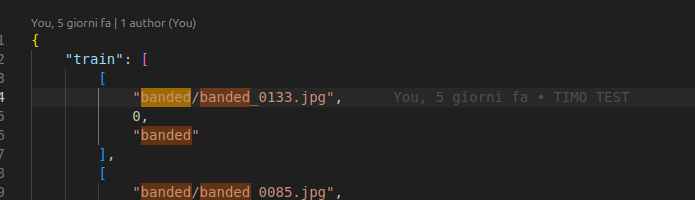
\includegraphics[width=0.5\textwidth]{TrainEx.png}
    \caption{Esempio di immagine dal training set (ipoteticamente dal dataset DTD, ad es. una texture "interlacciata").}
    \label{fig:train_ex}
\end{figure}

\subsection{Validation Set}
Il validation set è utilizzato per scopi intermedi, come l'ottimizzazione di iperparametri o la selezione di strategie, prima della valutazione finale sul test set.

\textbf{Utilizzo nel codice:}
\begin{enumerate}
    \item \textbf{Estrazione delle Feature Visive}: Similmente al training set, le feature visive delle immagini del validation set vengono estratte usando \texttt{clip\_model.encode\_image(images)} e salvate su disco. Questo è gestito dalla funzione \texttt{extract\_val\_test\_feature(cfg, "val", ...)} in \texttt{extract\_features\_all.py}. I file salvati sono tipicamente \texttt{val\_f.pt} (features) e \texttt{val\_l.pt} (labels).
    \item \textbf{Caricamento in \texttt{main.py}}: Queste feature vengono caricate in \texttt{main.py} tramite \texttt{loda\_val\_test\_feature(cfg, "val")}.
    \item \textbf{Ottimizzazione/Ricerca}: Nel caso di TIMO-S (TIMO con Search), il validation set (\texttt{val\_features}, \texttt{val\_labels}) è utilizzato dalla funzione \texttt{image\_guide\_text\_search} per ottimizzare o cercare i parametri migliori per la guida delle feature testuali da parte delle feature immagine.
\end{enumerate}

\subsection{Test Set}
Il test set è utilizzato esclusivamente per la valutazione finale delle prestazioni del modello. È fondamentale che questo set non venga utilizzato durante nessuna fase di training o ottimizzazione per garantire una stima imparziale della capacità di generalizzazione del modello.

\textbf{Utilizzo nel codice:}
\begin{enumerate}
    \item \textbf{Estrazione delle Feature Visive}: Le feature visive delle immagini del test set vengono estratte e salvate in modo analogo al validation set, utilizzando la funzione \texttt{extract\_val\_test\_feature(cfg, "test", ...)} in \texttt{extract\_features\_all.py}. I file salvati sono tipicamente \texttt{test\_f.pt} e \texttt{test\_l.pt}.
    \item \textbf{Caricamento in \texttt{main.py}}: Le feature del test set vengono caricate tramite \texttt{loda\_val\_test\_feature(cfg, "test")} (o \texttt{"val"} per ImageNet).
    \item \textbf{Valutazione Finale}: Le prestazioni di TIMO, TIMO-S e dei metodi baseline (Tip-Adapter, APE, GDA-CLIP) sono calcolate utilizzando le feature del test set (\texttt{test\_features}, \texttt{test\_labels}) e le rispettive strategie di classificazione. Le metriche (tipicamente l'accuracy) vengono poi registrate e salvate in \texttt{outputs/results.csv}.
\end{enumerate}
La Figura \ref{fig:test_ex} mostra un esempio di immagine che potrebbe appartenere al test set del dataset DTD.

\begin{figure}[h!]
    \centering
    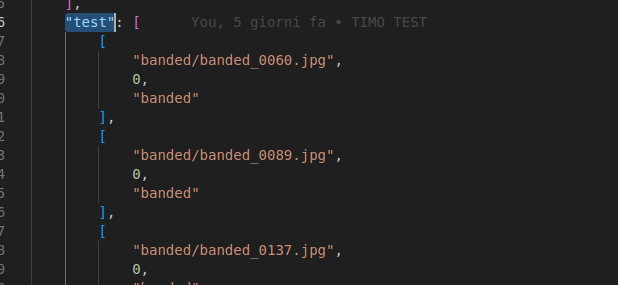
\includegraphics[width=0.5\textwidth]{TestEx.png}
    \caption{Esempio di immagine dal test set (ipoteticamente dal dataset DTD, ad es. una texture "punteggiata").}
    \label{fig:test_ex}
\end{figure}

\section{Estrazione e Caricamento delle Feature}
Un passaggio preliminare fondamentale nel flusso di lavoro di TIMO è l'estrazione delle feature, sia visive che testuali, che vengono poi salvate e caricate per l'elaborazione successiva. Questo approccio evita di dover rieseguire l'estrazione, computazionalmente onerosa, ad ogni esecuzione.

\subsection{Estrazione delle Feature (\texttt{extract\_features\_all.py})}
Il file \texttt{extract\_features\_all.py} è responsabile della generazione e del salvataggio di tutte le feature necessarie.
\begin{itemize}
    \item \textbf{Feature Visive}:
        \begin{itemize}
            \item \texttt{extract\_few\_shot\_feature}: Estrae feature dalle immagini del training set (few-shot), applica augmentation e le salva come \texttt{cache\_keys} e \texttt{cache\_values}.
            \item \texttt{extract\_val\_test\_feature}: Estrae feature dalle immagini dei set di validazione e test e le salva.
        \end{itemize}
    \item \textbf{Feature Testuali}:
        \begin{itemize}
            \item \texttt{extract\_text\_feature} e \texttt{extract\_text\_feature\_all}: Generano embedding testuali per ogni classe. Questo processo coinvolge:
                \begin{enumerate}
                    \item Nomi delle classi (es. dal dataset).
                    \item Template di prompt (es. "una foto di una {}").
                    \item Eventuali prompt aggiuntivi da file JSON (es. prompt generati da GPT o specifici del dataset come CuPL, specificati in \texttt{dataset.cupl\_path}).
                \end{enumerate}
                Questi testi vengono tokenizzati e passati all'encoder testuale di CLIP (\texttt{clip\_model.encode\_text}) per ottenere gli embedding, che vengono poi normalizzati e salvati (es. \texttt{text\_weights\_cupl\_t\_all.pt}).
        \end{itemize}
\end{itemize}
La Figura \ref{fig:feature_extraction} illustra schematicamente il processo di estrazione delle feature.

\begin{figure}[h!]
    \centering
    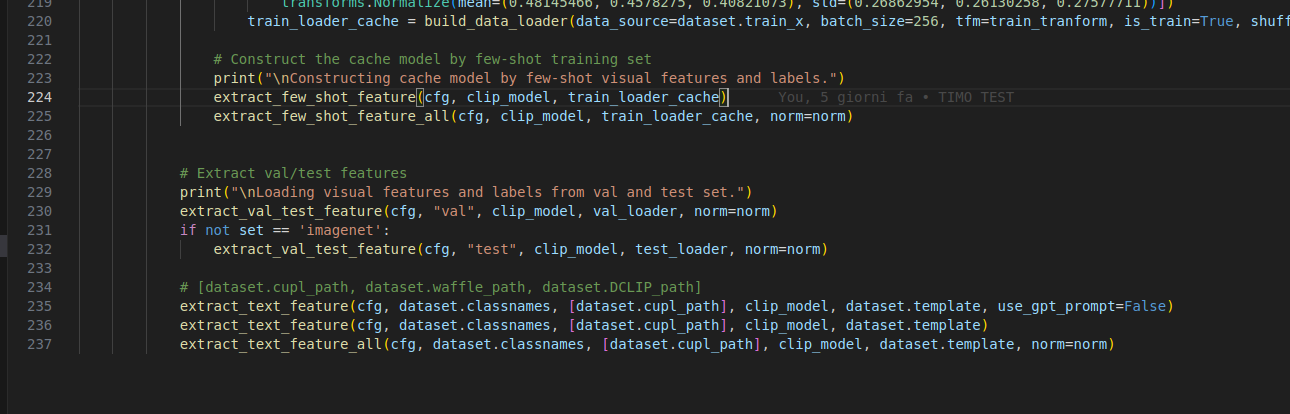
\includegraphics[width=0.7\textwidth]{FeatureExtract.png}
    \caption{Processo di estrazione delle feature visive e testuali utilizzando CLIP.}
    \label{fig:feature_extraction}
\end{figure}

\subsection{Caricamento delle Feature (\texttt{main.py})}
Il file \texttt{main.py} inizia caricando le feature pre-estratte e salvate nella directory \texttt{cache\_dir}.
\begin{itemize}
    \item \textbf{Feature Testuali}: Caricate da file \texttt{.pt}, ad esempio \texttt[breakable]{clip\_weights\_cupl\_all = torch.load(cfg['cache\_dir'] + "/text\_weights\_cupl\_t\_all.pt")}. Queste possono essere ulteriormente processate (es. media sui prompt) per ottenere i pesi del classificatore testuale di CLIP.
    \item \textbf{Feature del Training Set (Cache Model)}: Caricate tramite \texttt[breakable]{cache\_keys, cache\_values = load\_few\_shot\_feature(cfg)}.
    \item \textbf{Feature dei Set di Validazione e Test}: Caricate tramite \texttt[breakable]{val\_features, val\_labels = loda\_val\_test\_feature(cfg, "val")} e \texttt{test\_features, test\_labels = loda\_val\_test\_feature(cfg, "test")}.
\end{itemize}
La Figura \ref{fig:feature_loading} illustra il caricamento delle feature pre-calcolate.

\begin{figure}[h!]
    \centering
    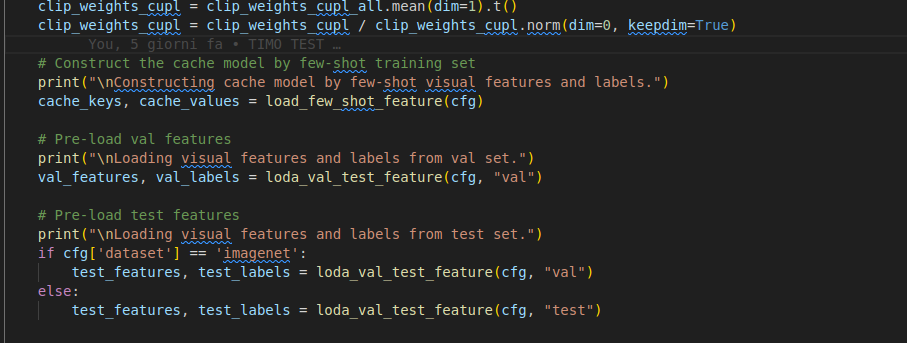
\includegraphics[width=0.7\textwidth]{FeatureLoading.png}
    \caption{Caricamento delle feature pre-estratte in \texttt{main.py}.}
    \label{fig:feature_loading}
\end{figure}

\section{Funzionamento di TIMO}
Una volta caricate tutte le feature necessarie, TIMO procede con il suo meccanismo di fusione e classificazione.

\subsection{Image-Guided Text (IGT)}
Un aspetto centrale di TIMO sembra essere la capacità di utilizzare le poche feature visive del training set per "guidare" o raffinare le feature testuali.
\begin{enumerate}
    \item \textbf{Creazione di "Image Weights"}: Dalle \texttt{cache\_keys} (feature visive del training set), vengono calcolati dei pesi medi per immagine per ogni classe (\texttt{image\_weights}). Questi rappresentano una sorta di prototipo visivo per ciascuna classe, basato sui pochi esempi disponibili.
    \item \textbf{Guida delle Feature Testuali}: La funzione \texttt{image\_guide\_text} (e la sua variante con ricerca \texttt{image\_guide\_text\_search} usata in TIMO-S) prende in input le feature testuali originali (es. \texttt{clip\_weights\_cupl\_all}) e i pesi delle immagini (\texttt{image\_weights}) per produrre delle feature testuali raffinate (\texttt{clip\_weights\_IGT}). Viene calcolato anche un \texttt{matching\_score}
\end{enumerate}

\subsection{Classificazione e Valutazione}
Con le feature testuali raffinate (\texttt{clip\_weights\_IGT}) e, in alcuni casi, le feature testuali originali e il \texttt{matching\_score}, TIMO esegue la classificazione sulle feature del test set.
\begin{itemize}
    \item \textbf{TIMO}: Utilizza \texttt{clip\_weights\_IGT}, \texttt{clip\_weights\_cupl\_all} e \texttt{matching\_score} per la classificazione. La funzione \texttt{TIMO(...)} in \texttt{main.py} implementa questa logica.
    \item \textbf{TIMO-S}: Simile a TIMO, ma \texttt{clip\_weights\_IGT} e \texttt{matching\_score} sono ottenuti tramite una fase di ricerca (\texttt{image\_guide\_text\_search}) che utilizza il validation set per ottimizzare i parametri della guida.
\end{itemize}
Le prestazioni (accuracy) vengono calcolate confrontando le predizioni con le \texttt{test\_labels}. I risultati vengono poi salvati, ad esempio in un file CSV (\texttt{outputs/results.csv}).

\section{Esempio con il Dataset DTD (Describable Textures Dataset)}
Il Describable Textures Dataset (DTD) è un dataset di immagini di texture, ed è uno dei dataset supportati da TIMO (come indicato in \texttt{datasets/\_\_init\_\_.py} e utilizzato in \texttt{extract\_features\_all.py}).

Il flusso di lavoro con DTD sarebbe il seguente:
\begin{enumerate}
    \item \textbf{Setup del Dataset}:
        \begin{itemize}
            \item Le immagini si trovano in \texttt{\$DATA/dtd/images/}.
            \item Le etichette e i nomi delle classi sono in \texttt{\$DATA/dtd/labels/}.
            \item La suddivisione in train, validation e test è definita nel file JSON \texttt{\$DATA/dtd/split\_zhou\_DescribableTextures.json}. Il caricamento e la gestione di queste suddivisioni sono gestiti dalla classe \texttt{DescribableTextures} in \texttt{datasets/dtd.py} (non fornito, ma deducibile da \texttt{datasets/\_\_init\_\_.py}) e dalle utility in \texttt{datasets/utils.py}.
        \end{itemize}
    \item \textbf{Estrazione Feature (come da Sezione 3 e 4.1)}:
        \begin{itemize}
            \item \textbf{Training (Few-Shot)}: Un piccolo numero di immagini per ogni classe di texture (es. "banded", "blotchy", "braided", come visibile in \texttt{TrainEx.png} che potrebbe rappresentare una texture "interlacciata" o "a rete") viene selezionato dal set di training di DTD. Le loro feature visive vengono estratte e salvate come \texttt{cache\_keys} e \texttt{cache\_values}.
            \item \textbf{Validation}: Le immagini dal set di validazione di DTD vengono processate per estrarre \texttt{val\_features} e \texttt{val\_labels}.
            \item \textbf{Test}: Le immagini dal set di test di DTD (es. una texture "punteggiata" come in \texttt{TestEx.png}) vengono processate per estrarre \texttt{test\_features} e \texttt{test\_labels}.
            \item \textbf{Testuali}: Le feature testuali per le classi di DTD (es. "banded", "blotchy", etc.) vengono estratte usando i template e i prompt specifici per DTD.
        \end{itemize}
    \item \textbf{Esecuzione di TIMO (come da Sezione 4.2 e 5)}:
        \begin{itemize}
            \item Le feature estratte vengono caricate.
            \item TIMO utilizza le feature del training set di DTD per raffinare le feature testuali delle texture.
            \item Il modello viene valutato sulle feature del test set di DTD per misurare la sua capacità di classificare correttamente le texture mai viste prima, basandosi su pochi esempi.
        \end{itemize}
\end{enumerate}
Questo processo permette a TIMO di adattarsi e classificare efficacemente le diverse texture presenti nel dataset DTD, anche con un supporto di training limitato. I risultati, inclusa l'accuracy media per il dataset DTD con un certo numero di shot e seed, vengono salvati nel file \texttt{outputs/results.csv}.

Come possibile vedere dalle immagini \texttt{TrainEx.png} e \texttt{TestEx.png}, gli autori di TIMO hanno inserito le stesse classi sia nel training set che nel test set (ovviamente non inserendo le stesse immagini).

\section{Considerazioni per il nostro lavoro}

Dato che il nostro lavoro si basa su TIMO, è fondamentale comprendere a fondo il suo funzionamento e replicarlo. Il nostro task prevedere di effettuare FSL con k=[1,2,4,8,16]

\subsection{Artgraph\_Artist}

In questo caso le classi sono gli artisti e le immagini sono le loro opere. Dobbiamo organizzare il dataset affinchè sia compatibile con TIMO e con il task di few-shot learning. Per questo motivo viene proposta la seguente divisione in training, validation e test set:
\begin{itemize}
    \item \textbf{Test set}: Dato che dobbiamo eseguire task fino a 16-shot, il test set deve contenere almeno 16 immagini per ogni artista. Per questo motivo, il test set è composto da 16 immagini per ogni artista. Le immagini sono state scelte in modo casuale tra le opere di ogni artista.
    \item \textbf{Training e validation set}: Per il training e il validation set si potrebbero inserire rispettivamente 10 e 5 immagini per artista. 
    \item \textbf{Artisti con poche opere}: Gli artisti che non presentano opere sufficienti per creare i set verranno esclusi dal dataset.
\end{itemize}

\subsection{Artgraph\_Style}
In questo caso le classi sono gli stili e le immagini sono le opere. Dobbiamo organizzare il dataset affinchè sia compatibile con TIMO e con il task di few-shot learning. Prendiamo le 10 classi più rappresentate e creiamo i set di training, validation e test come segue:
\begin{itemize}
    \item \textbf{Test set}: Dato che dobbiamo eseguire task fino a 16-shot, il test set deve contenere almeno 16 immagini per ogni stile. Un buon approcio potrebbe essere quello di prendere tutti gli artisti che partecipano a quello stile e prendere 5 immagini di quell'artista in quello stile. (senza alcun problema si dovrebbero raggiungere le 16 immagini per stile)
    \item \textbf{Training e validation set}: Per il training e il validation set si potrebbero inserire rispettivamente 20 e 10 immagini per stile randomicamente 
    \item \textbf{Stili con poche opere}: Gli stili che non presentano opere sufficienti per creare i set verranno esclusi dal dataset.
\end{itemize}

\end{document}

